\section{Architettura lato Client (GUI)}
\subsection{Tecnologie utilizzate}
\subsubsection{React.js}
React è un framework open-source che permette di implementare applicazioni web seguendo i principi della
programmazione ad oggetti. In modo particolare risulta essenziale comprendere tre concetti chiave:
\begin{itemize}
    \item \textbf{JSX}\\
    JSX è un'estensione della sintassi di JavaScript.\newline
    Permette di unire gli aspetti di html come linguaggio di template agli aspetti di JavaScript come linguaggio di scripting in una forma che ne aumenta semplicità e leggibilità.\newline
    Gli elementi JSX vengono utilizzati nelle definizioni delle funzioni di rendering (che verranno trattate a breve) semplificando la costruzione della user interface.\newline
    Attraverso JSX possiamo richiamare un componente React tramite con un meccanismo analogo ai tag in html.
    \item  \textbf{Componenti}\\
    Attraverso un componente andiamo a definire quella che risulta essere a tutti gli effetti una classe.\newline
    Il nostro componente, definito da uno o più costruttori, contiene uno stato; questo stato verrà mantenuto, ed eventualmente aggiornato, durante tutto il ciclo di vita (lifecycle) del componente.\newline
    È possibile ricevere dati ed istruzioni da altri componenti attraverso le props.\newline
    \item \textbf{Stato}\\
    Lo stato un insieme di proprietà di un componente.\newline
    Queste proprietà possono variare a seguito dell'interazione con altri componenti o come azione del componente stesso nel caso esso esegua delle azioni a cadenza temporale.\newline
    In React inoltre lo stato risulta fondamentale ai fini di ottenere un rendering a schermo performante; ogni componente React infatti deve obbligatoriamente definire una funzione \emph{render()}.\newline
    Attraverso di essa verrà ritornato il contenuto da renderizzare a schermo.\newline
    React cambierà il contenuto a schermo (consumando quindi risorse) solamente quando vi saranno delle modifiche nel contenuto ritornato dalla funzione render(); utilizzando dunque le proprietà che definiscono lo stato del componente all'interno della funzione render() del componente stesso riusciremo a ridurre al minimo indispensabile il numero di volte in cui l'applicazione verrà renderizzata, riflettendo i cambiamenti di stato del componente.
\end{itemize}
\begin{figure}[H]
    \caption{Logo di React.js}
    \centering
    
\includegraphics[width=40mm]{img/react_logo.png}
    \label{fig:react_logo}
\end{figure}

\subsection{Struttura del Client}
Il client si occupa di mostrare a schermo i dati relativi alle soluzioni di viaggio e permette di monitorare la situazione di un determinato treno o di una stazione.
\subsubsection{Stato e Request}
Per recuperare i dati vengono effettuate delle request di tipo GET al server.\newline
Gli oggetti in formato json che vengono ritornati come response vengono incapsulati all'interno di uno \textit{state} di React.
\begin{minted}{js}
this.state = {trainInfo: {name: "", departure:{}, arrival:{}, lastStop:{}}}
\end{minted}

\noindent Il motore del framework per sua natura si occupa di renderizzare nuovamente tutta la pagina in caso di cambiamenti all'interno dello stato.
Grazie a questo meccanismo non è necessario fare altro oltre che assegnare il valore di risposta allo state corretto. Per effettuare le richieste è stata utilizzata la libreria JQuery.\newline
Il codice che segue è la funzione che si occupa di effettuare una request per recuperare lo stato di un determinato treno:
\begin{minted}{js}
    $.get(SERVER_URL + "/real-time-train-info?trainNumber=" + trainID)
            .done((result) => {
                console.log("GET Request Done")
                this.setState({trainInfo: result});
            })
            .fail((result) => {
                console.log("An error occurred: " + result);
            })
\end{minted}

\noindent Il codice utilizzato per recuperare lo stato di una stazione o le soluzioni a partire da determinati valori di input è strutturato esattamente allo stesso modo.\newline

\noindent Per effettuare il monitoraggio di treni e stazione è stata utilizzata la funzione \textit{setInterval}, che permette di eseguire un handler ogni \textit{"x"} millisecondi. L'handler non è altro che la funzione che si occupa di effettuare la request al server ed aggiornare lo stato.\newline
Per interrompere il monitoraggio si può utilizzare la funzione \textit{clearInterval}, la quale permette di eliminare il timer introdotto precedentemente.\newline

\noindent React inoltre mette a disposizione delle funzioni, \textit{componentDidMount} e \textit{componentWillUnmount} che tornano molto utili in questo caso. Ogni volta che un determinato componente viene renderizzato viene eseguita \textit{componentDidMount}, ogni volta che viene rimosso viene invece eseguita la \textit{componentWillUnmount}. Quest'ultima è un posto perfetto per inserire una \textit{clearInterval}, che si occupa di eliminare il timer impostato utilizzando \textit{setInterval} qualora esistesse ancora nel momento in cui per esempio si cambia pagina.

\subsubsection{Schermate del Client}
La GUI è composta da quattro schermate. Dalla Homepage è possibile cliccare dei bottoni per effettuare il redirect alla pagina interessata.\newline
Le tre pagine più importanti sono:
\begin{itemize}
    \item \textbf{Schermata di visualizzazione delle soluzioni di viaggio:}\newline Da questa pagina è possibile ottenere le soluzioni di viaggio a partire da alcuni parametri che è possibile impostare attraverso un form dedicato.\newline
    Il form permette di inserire stazione di partenza, stazione di arrivo, data e ora. Verranno quindi mostrare le cinque soluzioni più vicine all'orario impostato.
    \begin{figure}[H]
        \caption{Schermata di visualizzazione delle soluzioni di viaggio}
        \centering
        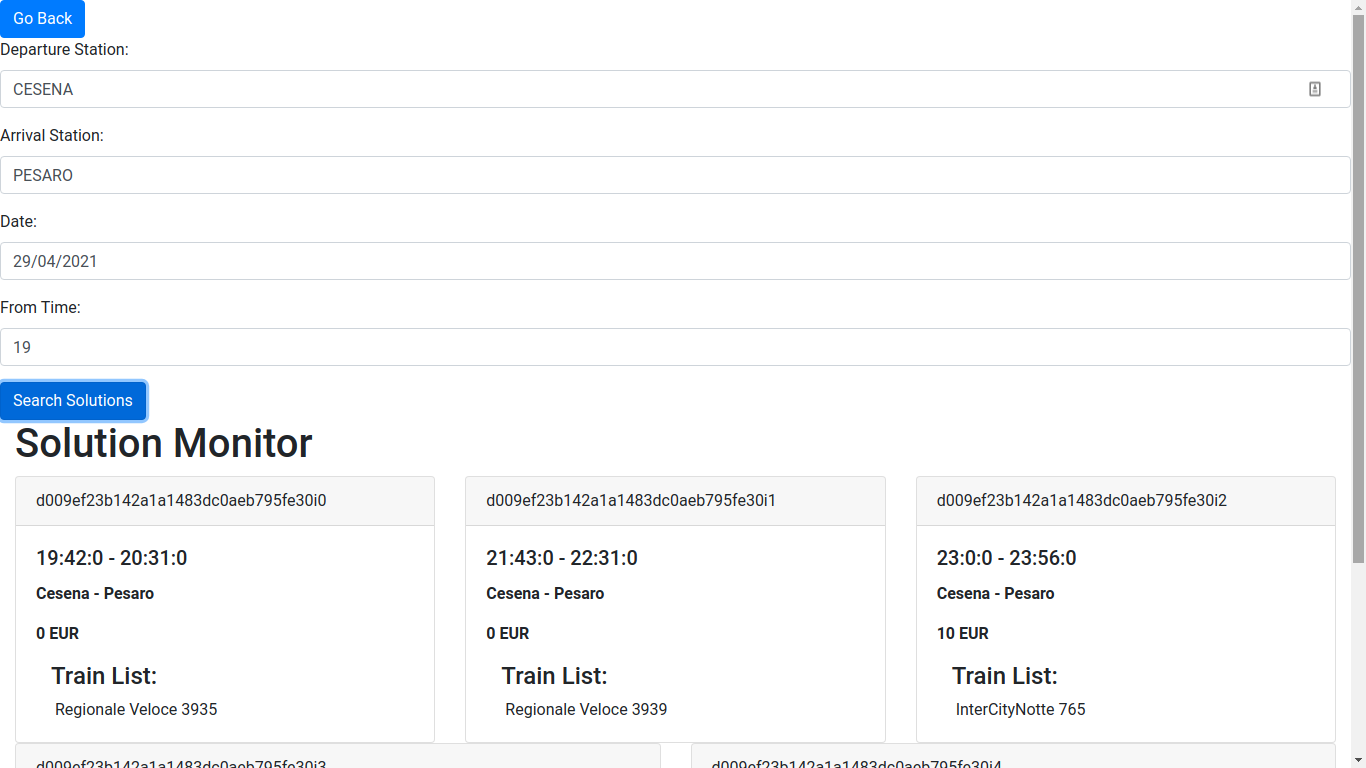
\includegraphics[width=150mm]{img/screenshot/solutions.png}
        \label{fig:solutions}
    \end{figure}
    \item \textbf{Schermata di visualizzazione delle Info di un treno:}\newline Da questa pagina è possibile monitorare la situazione di un determinato treno.\newline
    Il form permette di inserire il codice del treno che si desidera tenere sotto osservazione.
    Verrà quindi mostrata la situazione del treno in tempo reale.\newline
    In qualsiasi momento è possibile interrompere il monitoraggio tramite l'apposito pulsante \textit{"Stop Monitoring"} o farlo ripartire se fermo cliccando \textit{"Start Monitoring"}.
    \begin{figure}[H]
        \caption{Schermata di visualizzazione delle Info Treno}
        \centering
        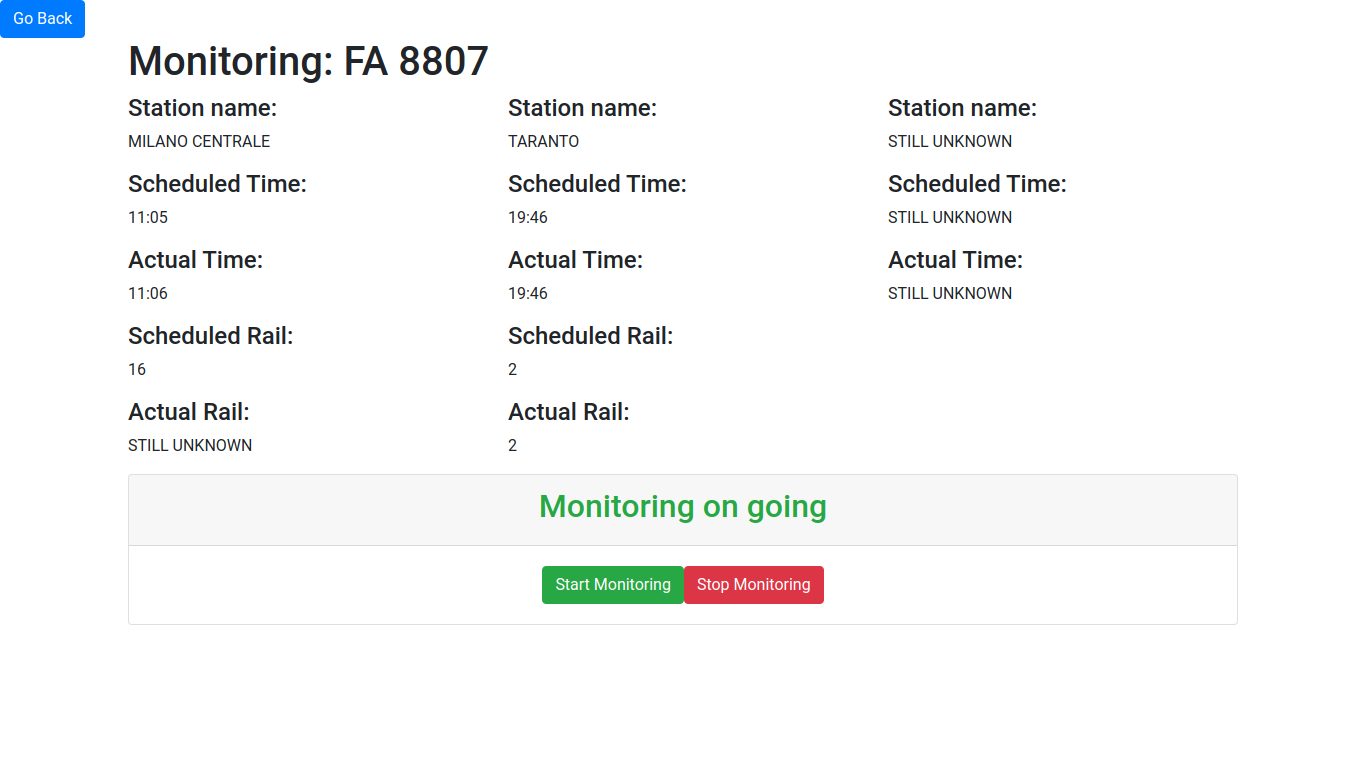
\includegraphics[width=150mm]{img/screenshot/train.png}
        \label{fig:train_info}
    \end{figure}
     \item \textbf{Schermata di visualizzazione delle Info di una stazione:}\newline Da questa pagina è possibile monitorare la situazione di una determinata stazione.\newline
    Il form permette di inserire il codice della stazione che si desidera tenere sotto osservazione.
    Verrà quindi mostrata la situazione della stazione in tempo reale.\newline
    In qualsiasi momento è possibile interrompere il monitoraggio tramite l'apposito pulsante \textit{"Stop Monitoring"} o farlo ripartire se fermo cliccando \textit{"Start Monitoring"}.
    \begin{figure}[H]
        \caption{Schermata di visualizzazione delle Info Stazione}
        \centering
        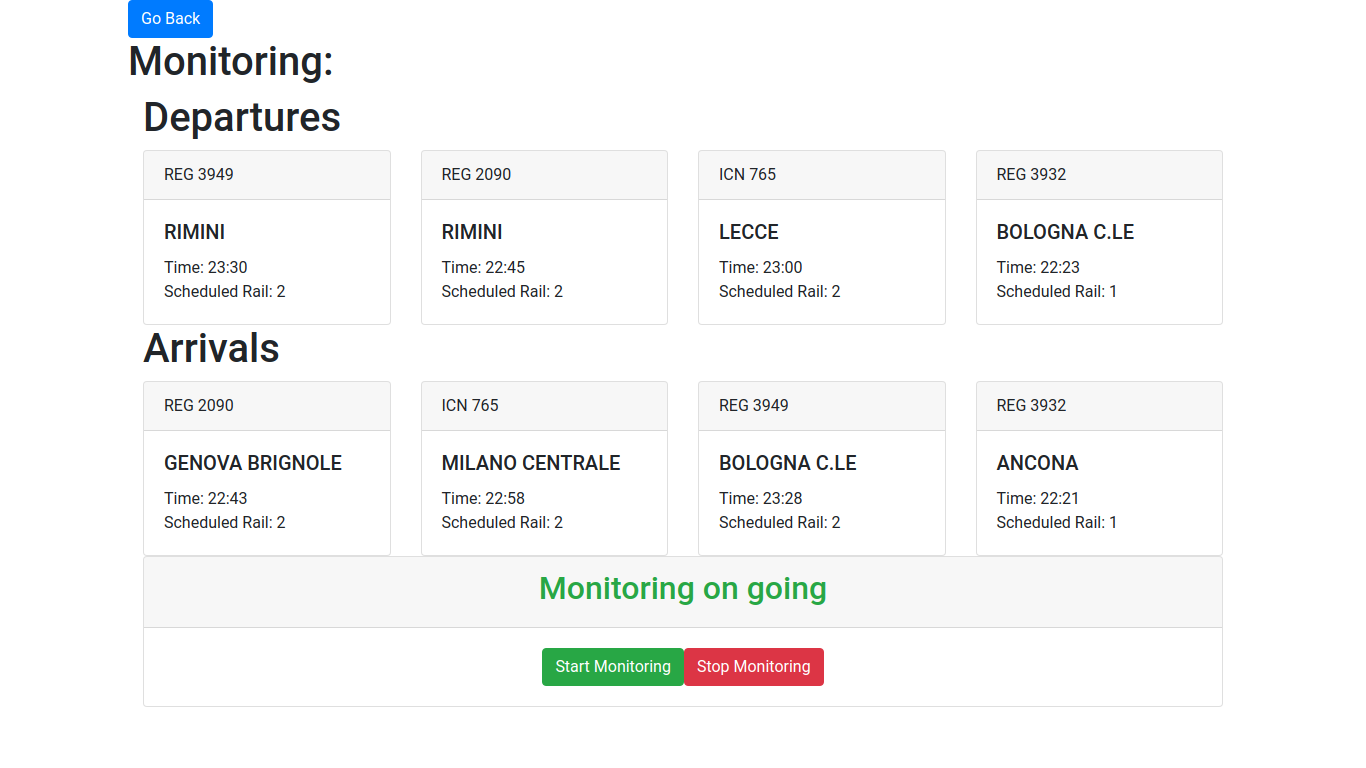
\includegraphics[width=160mm]{img/screenshot/station.png}
        \label{fig:station_info}
    \end{figure}
\end{itemize}
